\section{Schritt 4}
Die nächste Erweiterung der Anwendung bildet die Konstruktion der $A^{S}_{k,q}$ für gegebene Primzahlen (k, q) und eine Gruppe S.\\
\\
Die in Schritt 3 berechnete Erzeugermatrix wird nun weiterverwendet und auf die einzelnen Repräsentanten angewendet. Getestet wird hierbei, ob das Ergebnis in der gleichen Gruppe liegt. Dieser Fall trifft zu, wenn das Ergebnis den Repräsentanten selbst oder ein Vielfaches darstellt. \\
Trifft dies nicht zu, ist das Ergebnis ein Element einer anderen Gruppe. Sind alle Gruppen gefunden, startet die Suche nach Zyklen. Getestet wird hierbei, ob diese verschiedenen Gruppen in Kombination mit der Erzeugermatrix verkettet werden können. Ein Beispiel für einen solchen Zyklus wäre, wenn fortlaufend aus einem Element aus r0 ein Element der Gruppe r2 erzeugt wird, aus r2 eines der Gruppe r8 und aus r8 wiederum ein Element von r0.\\
Ist ein solcher Zyklus gefunden, werden alle entsprechenden Spalten addiert und ergeben einen gemeinsamen Vektor C. Dieser enthält somit alle Elemente innerhalb einer Gruppe.\\
\\
Folgende Ausgaben ergeben sich beim Test für die Werte q,k,b = 3:

\begin{figure}
	\centering
	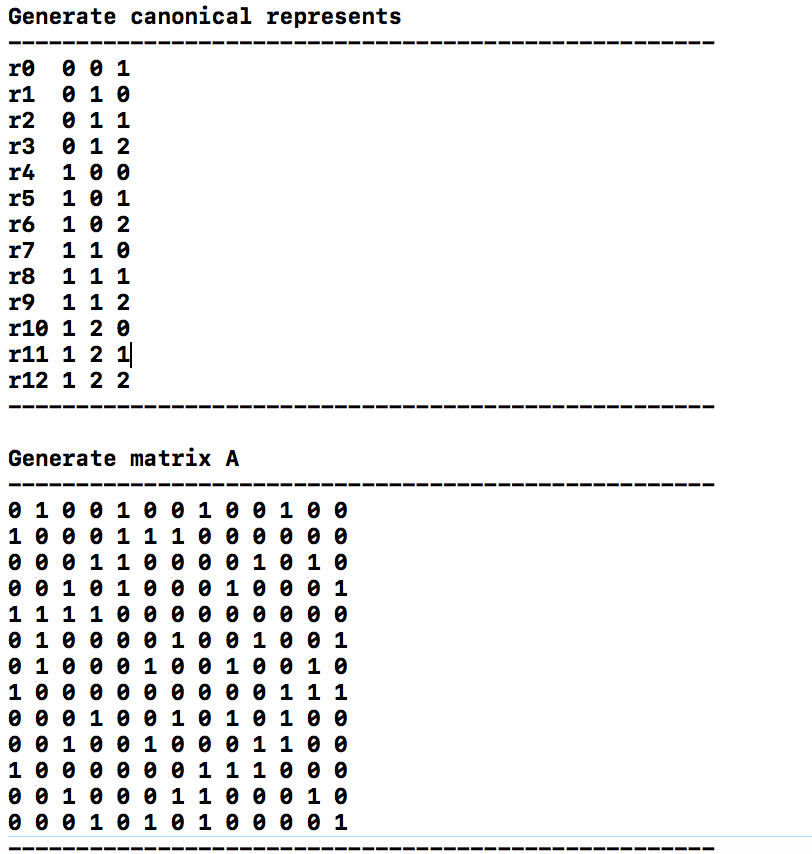
\includegraphics[width=0.5\textwidth]{Pictures/step4_generateMatrix}
	\caption{Berechnung der Matrix A über Repräsentanten}
\end{figure}

\begin{figure}
	\centering
	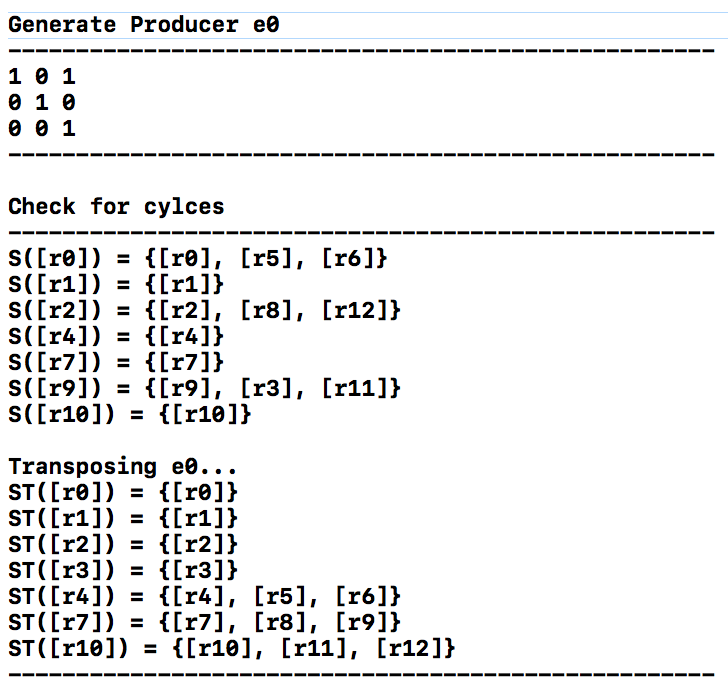
\includegraphics[width=0.5\textwidth]{Pictures/step4_cycle_check}
	\caption{Erzeugermatrix e0 und die Suche nach Zyklen}
\end{figure}

\begin{figure}
	\centering
	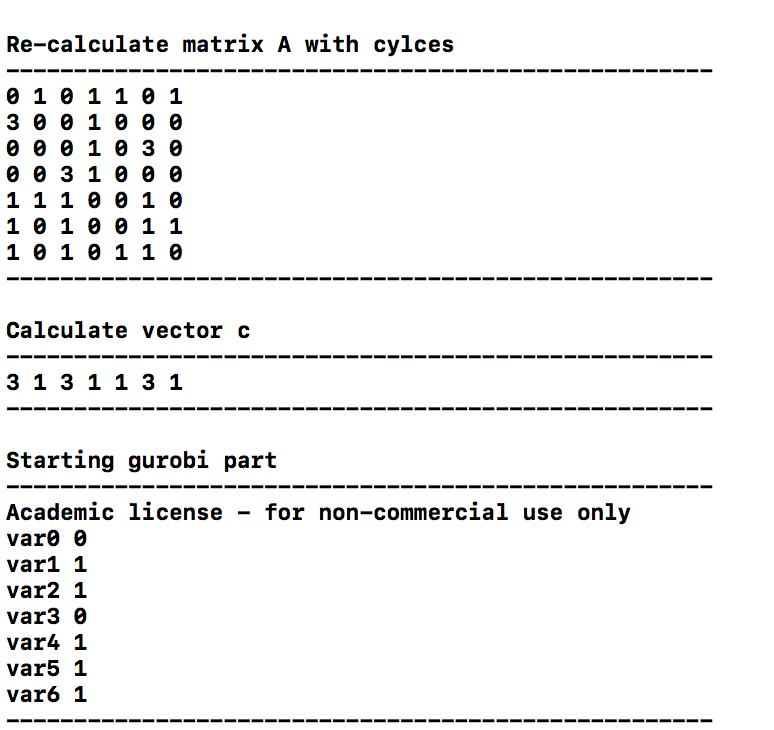
\includegraphics[width=0.5\textwidth]{Pictures/step4_recalcA}
	\caption{Erneute Berechnung von A und Gurobi}
\end{figure}

\begin{figure}
	\centering
	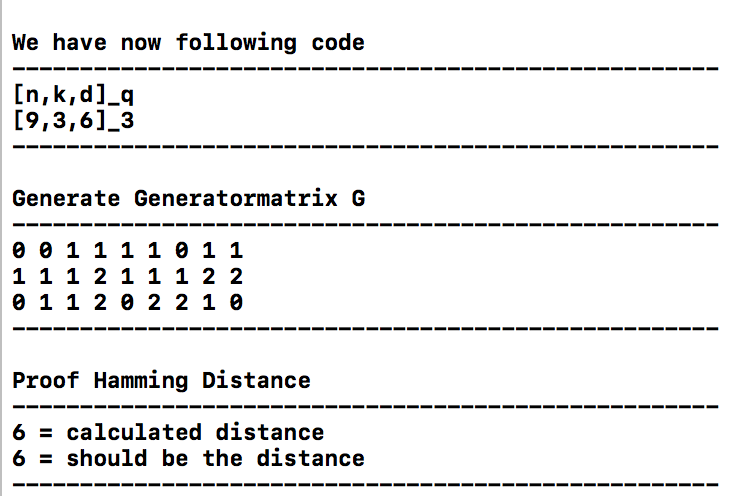
\includegraphics[width=0.5\textwidth]{Pictures/step4_end}
	\caption{Code C, Generatormatrix G und Hamming-Test}
\end{figure}
\newpage